\chapter{Exclusion mutuelle}
\startchapter

\lettrine[lines=4]{L}{orsque} des tâches entrent en conflit pour l'accès à une ressource unique et non partageable, il devient nécessaire de limiter l'accès à la ressource à une seule tâche au plus et à chaque instant.  La ressource, qui ne peut être utilisée que par une seule tâche à la fois, peut être un périphérique ou une variable mise à jour par plusieurs tâches. Cette ressource, physique ou logique, est appelée {\em ressource critique}. Lorsqu'il s'agit de réaliser l'exclusion mutuelle entre des tâches dans un fragment de leur code, on appelle ces fragments des {\em sections critiques} plutôt que des ressources critiques. Remarquons que l'accès à un périphérique se fait aussi par un fragment de code.
\par
Illustrons le problème de l'exclusion mutuelle par un exemple.  Soient deux tâches $T_1$ et $T_2$ qui incrémentent une variable partagée $x$, initialisée à $0$.  Il est parfaitement raisonnable que la valeur finale après l'exécution de $T_1$ et de $T_2$ soit 1 ou 2.
Ceci est lié au fait que l'énoncé d'affectation n'est pas toujours implémenté comme une opération indivisible.  En effet, cet énoncé peut se traduire en 3 instructions assembleurs
\begin{displaymath}
\begin{array}{ccll}
       &                             & (1) & x \rightarrow \mbox{registre} \\
x:=x+1 & \Rightarrow & (2) & \mbox{inc registre} \\
       &                             & (3) & \mbox{registre} \rightarrow x
\end{array}
\end{displaymath}
Sous sa forme en assembleur, l'énoncé d'affectation peut être interrompu à deux endroits avant de compléter son exécution.  Pour résoudre le problème, il faut ordonner l'utilisation de la ressource critique.  Ainsi, si une tâche $T_i$ utilise la ressource et si une autre tâche $T_j$ désire elle aussi l'utiliser, alors $T_j$ doit
être retardée tant que $T_i$ ne la libère pas.
\noindent
Avant d'apporter une solution au problème de l'exclusion mutuelle, regardons quelques embûches à éviter.
\begin{enumerate}
\item {\em Il ne doit pas y avoir d'interblocage}.  La ressource critique doit être accessible.
\item {\em Il faut éviter la famine}.  Considérons la situation décrite à la figure~\ref{figex:famine} illustrant une ressource partagée entre 3 tâches.
 Si la situation représentée persiste, c.-à-d. que $T_1$ et $T_3$ utilisent à nouveau abondamment la ressource, $T_2$ n'accédera jamais à ressource et restera indéfiniment retardée.
\end{enumerate}

\begin{figure}[tb]
\figcaption{figex:famine}{Situation de famine}
\begin{center}
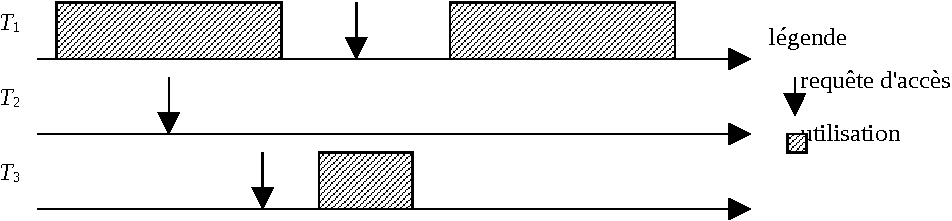
\includegraphics[width=.9\textwidth]{FigFamine}
\end{center}
\vspace{-.2cm}
\rule{\textwidth}{0.01in}
\end{figure}

\section{Classification des solutions}
Les différentes solutions apportées au problème de l'exclusion mutuelle que nous verrons peuvent être classées selon l'attente des tâches pour la ressource et selon l'environnement sur lequel ces tâches s'exécutent.
\par
L'attente des tâches à une ressource critique peut se caractériser suivant l'ordre dans lequel les tâches accèdent à la ressource.
\begin{itemize}
\item[(a)] L'attente est {\em PAPS} (FIFO en anglais) lorsque les tâches l'accèdent selon leur ordre d'arrivée.
\item[(b)] L'attente est {\em linéaire} lorsqu'une tâche ne peut accéder deux fois la ressource alors qu'une autre tâche est en attente.
Une tâche qui a obtenu la ressource et qui la redemande ne peut pas dépasser une tâche qu'elle a trouvé en attente auparavant.
\item[(c)] L'attente est {\em bornée par une fonction} $f(n)$ où $n$ est le nombre de tâches participantes à l'exclusion mutuelle, si une tâche désireuse d'accéder à la ressource ne peut pas se laisser dépasser que par un maximum de $f(n)$ tâches.
\item[(d)] L'attente est {\em finie} si elle n'est pas bornée mais pas infinie. Une tâche atteindra la ressource après un temps fini.  Il n'y a donc pas de famine.
\end{itemize}
\par
L'environnement joue un rôle dans la façon de résoudre le problème de l'exclusion mutuelle.  Ainsi nous distinguons les solutions {\em centralisées} et les solutions {\em réparties}. On appelle une solution centralisée, une solution qui repose sur l'existence d'une mémoire centrale pouvant être accédée par toutes les tâches en lecture ou en écriture. On appelle une solution répartie, une solution où il n'y a plus de mémoire commune.
Dans ce dernier cas, chaque tâche possède une mémoire locale dans laquelle elle est la seule à pouvoir lire et écrire. Les tâches peuvent s'échanger des résultats uniquement par le biais de messages. Il se peut donc que lorsqu'une tâche obtient la valeur d'une variable que cette valeur ait été modifiée entre temps. {\em Il y a pas de perception d'un état global en répartie.}
Dans ce qui suit on s'intéresse à plusieurs solutions possibles afin de résoudre le problème de l'exclusion mutuelle dans un environnement centralisé. L'exclusion mutuelle en répartie sera traitée dans l'unité d'enseignement {\em Programmation répartie.}

\section{Solutions logicielles par attente active}
Quoiqu'il existe des solutions matérielles au problème de l'exclusion mutuelle ou encore des solutions fournies par le noyau du système d'exploitation sur lequel repose nos tâches, l'étude de solutions logicielles présente deux facettes intéressantes.  L'une des difficultés rencontrée en traitement parallèle est notre intuition inadéquate pour confronter les opérations parallèles et pour saisir leur interaction. Une raison importante d'aborder ces solutions logicielles est donc d'élucider, par le biais d'arguments plutôt détaillés, les notions d'exécution atomique et d'attente bornée.
Les descriptions des relations temporelles et du comportement du logiciel s'avèreront suffisantes pour montrer rigoureusement, et ceci sans introduire d'outil mathématique nouveau, les propriétés des algorithmes.

Les solutions apportées au problème de l'exclusion mutuelle doivent satisfaire les contraintes suivantes.
\begin{enumerate}
\item On ne fait aucune hypothèse à propos des instructions ni du nombre de processeurs dans l'environnement.
On suppose uniquement que les instructions assembleurs (telles que load, store, etc.) sont exécutées atomiquement.  Si deux de ces instructions sont exécutées simultanément, le résultat sera le même que si elles étaient exécutées l'une après l'autre dans un ordre inconnu à priori.
\item On ne fait aucune hypothèse sur les vitesses relatives des tâches.
\item Lorsqu'une tâche n'est pas dans sa section critique, elle ne doit pas empêcher les autres tâches d'entrer dans leur section critique.
\item On ne doit pas remettre indéfiniment la décision qui consiste à admettre l'une des tâche qui est en compétition pour l'accès à la section critique.
\end{enumerate}
\par
Nous nous attardons maintenant à présenter les premiers algorithmes pour assurer l'exclusion mutuelle.  Ces algorithmes sont basés sur le principe de {\em l'attente active}.  Une tâche peut boucler sur une condition et l'évaluer de manière répétitive jusqu'à ce qu'elle change d'état.
\par
Dans le cadre de ce cours, nous nous limitons aux algorithmes qui synchronisent seulement deux tâches.  La généralisation de ces algorithmes à $n$ tâches ne fait pas partie du cours.  La présentation de ces algorithmes suit le schéma donné sur la figure~\ref{algex:générale}.
Les parties {\em prélude} et {\em postlude} constituent le protocole que doivent suivre les deux tâches \ccode{T0} et \ccode{T1} pour respectivement pénétrer et sortir de leur section critique.  Les parties des tâches non comprises entre les parties prélude et postlude constituent la partie non-critique.

\begin{figure}[!ht]
\figcaption{algex:générale}{Schéma général des algorithmes d'exclusion mutuelle}
\begin{center}
\begin{tabular}{l}
\lstset{language=C++}
\begin{lstlisting}
// variables globales
void *T0(void *arg)
{
	while (true) {
		<prélude>
		<section critique>
		<postlude>
		<section non-critique>
	}
}

void *T1(void *arg)
{
	while (true) {
		<prélude>
		<section critique>
		<postlude>
		<section non-critique>
	}
}
\end{lstlisting}
\end{tabular}
\end{center}
\vspace{-.2cm}
\rule{\textwidth}{0.01in}
\end{figure}

\subsection*{Première tentative}
Le principe de la solution présentée sur l'algorithme~\ref{algex:tentative1} repose sur une variable booléenne appelée $occupe$ qui indique si l'une des tâches s'exécute en section critique.
Initialement, $occupe$ est positionné à faux.

\begin{algorithm}[!ht]
\caption{Première tentative d'exclusion mutuelle}\label{algex:tentative1}
\begin{center}
\begin{tabular}{l}
\lstset{language=C++}
\begin{lstlisting}
bool occupe = false;

void *T0(void *arg)
{
	while (true) {
		while (occupe)
			;
		occupe = true;
		/* section critique */
		occupe = false;
		/* section non-critique */
	}
}

void *T1(void *arg)
{
	while (true) {
		while (occupe)
			;
		occupe = true;
		/* section critique */
		occupe = false;
		/* section non-critique */
	}
}
\end{lstlisting}
\end{tabular}
\end{center}
\end{algorithm}

Malheureusement notre solution est incorrecte car on peut imaginer le scénario suivant.
\begin{center}
\begin{tabular}{cl}
$T_0$& lit $occupe$ à faux \\
$T_1$& lit aussi $occupe$ à faux \\
$T_1$& met $occupe$ à vrai \\
$T_1$& entre en section critique \\
$T_0$& met aussi $occupe$ à vrai \\
$T_0$& entre aussi en section critique. \\
\end{tabular}
\end{center}
Les deux tâches peuvent se retrouver simultanément en section critique.  Il n'y a donc pas d'exclusion mutuelle.

\subsection*{Deuxième tentative}
Notre deuxième tentative, algorithme ~\ref{algex:tentative2}, utilise une variable entière $tour$ qui indique l'identité de la tâche qui a l'autorisation d'accéder à la section critique.
Ainsi $T_i$ peut accéder à la section critique seulement si $tour$ est égale à $i$.

\begin{algorithm}[!ht]
\caption{Deuxième tentative d'exclusion mutuelle}\label{algex:tentative2}
\begin{center}
\begin{tabular}{l}
\lstset{language=C++}
\begin{lstlisting}
int tour = 0;  // ou 1

void *T0(void *arg)
{
	while (true) {
		while (tour != 0)
			;
		/* section critique */
		tour = 1;
		/* section non-critique */
	}
}

void *T1(void *arg)
{
	while (true) {
		while (tour != 1)
			;
		/* section critique */
		tour = 0;
		/* section non-critique */
	}
}
\end{lstlisting}
\end{tabular}
\end{center}
\end{algorithm}

Notre solution garantit qu'une seule tâche peut se trouver en section critique.  Cependant elle ne satisfait pas notre troisième contrainte.
Les tâches doivent exécuter leur section critique en alternance.
Une tâche peut donc attendre pour pénétrer en section critique alors que celle auquel le tour lui revient ne l'utilise pas et n'a peut-être plus l'intention de l'utiliser.
La plus lente des deux tâches impose son rythme à l'autre.  De plus, si une des deux tâches disparaît, l'autre attendra indéfiniment.

\subsection*{Troisième tentative}
Le problème avec notre solution précédente est lié au fait qu'elle tient compte de l'identité de la tâche qui peut accéder à la section critique sans considérer son état.
Pour remédier au problème, remplaçons la variable $tour$ de notre solution précédente par un vecteur de booléen $etat$ initialisé à faux.
Ainsi $etat[i]$ est vrai si $T_i$ est en section critique.
Malheureusement notre nouvelle solution, algorithme~\ref{algex:tentative3}, ne garantit plus l'exclusion mutuelle comme le montre la séquence qui suit.
\par\noindent
\begin{center}
\begin{tabular}{l}
$T_0$ exécute sa boucle et trouve $etat[1]$ à faux \\
$T_1$ exécute sa boucle et trouve aussi $etat [0]$ à faux \\
$T_0$ met $etat[0]$ à vrai et entre en section critique \\
$T_1$ met $etat[1]$ à vrai et entre aussi en section critique. \\
\end{tabular}
\end{center}
\par\noindent
Notre solution dépend des vitesses relatives des tâches.

\begin{algorithm}[!ht]
\caption{Troisième tentative d'exclusion mutuelle}\label{algex:tentative3}
\begin{center}
\begin{tabular}{l}
\lstset{language=C++}
\begin{lstlisting}
bool etat[2] = {false,false};

void *T0(void *arg)
{
	while (true) {
		while (etat[1])
			;
		etat[0] = true;
		/* section critique */
		etat[0] = false;
		/* section non-critique */
	}
}

void *T1(void *arg)
{
	while (true) {
		while (etat[0])
			;
		etat[1] = true;
		/* section critique */
		etat[1] = false;
		/* section non-critique */
	}
}
\end{lstlisting}
\end{tabular}
\end{center}
\end{algorithm}

\subsection*{Quatrième tentative}
Le problème avec notre troisième tentative provient du fait que l'une des tâches peut vérifier l'état de l'autre avant que cette dernière ait l'opportunité de modifier son état.  Corrigeons ce problème en déplaçant l'énoncé d'affectation comme l'illustre l'algorithme~\ref{algex:tentative4}.
Ainsi $etat[i]$ est vrai si $T_i$ désire accéder à la section critique.
\begin{algorithm}[!ht]
\caption{Quatrième tentative d'exclusion mutuelle}\label{algex:tentative4}
\begin{center}
\begin{tabular}{l}
\lstset{language=C++}
\begin{lstlisting}
bool etat[2] = {false,false};

void *T0(void *arg)
{
	while (true) {
		etat[0] = true;
		while (etat[1])
			;
		/* section critique */
		etat[0] = false;
		/* section non-critique */
	}
}

void *T1(void *arg)
{
	while (true) {
		etat[1] = true;
		while (etat[0])
			;
		/* section critique */
		etat[1] = false;
		/* section non-critique */
	}
}
\end{lstlisting}
\end{tabular}
\end{center}
\end{algorithm}

L'exclusion mutuelle est à présent garantie mais un autre problème surgit.
Si $T_0$ met $etat[0]$ à vrai et juste après $T_1$ met $etat[1]$ à vrai, alors $T_0$ et $T_1$ bouclent indéfiniment.
Si les deux tâches progressent simultanément dans leur prélude elles se bloquent mutuellement.
Chacune croit que l'autre est engagée dans sa section critique.
Ceci provient du fait que $T_i$ indique son intention d'entrer en section critique sans connaître l'intention de l'autre.

\subsection*{Cinquième tentative}
Modifions notre précédente tentative de manière à obliger une tâche à renoncer temporairement à son désir de pénétrer en section critique si l'autre tâche désire elle aussi y entrer.
Cette nouvelle tentative est donnée par l'algorithme~\ref{algex:tentative5}.
\begin{algorithm}[!ht]
\caption{Cinquième tentative d'exclusion mutuelle}\label{algex:tentative5}
\begin{center}
\begin{tabular}{l}
\lstset{language=C++}
\begin{lstlisting}
bool etat[2] = {false,false};

void *T0(void *arg)
{
	while (true) {
		etat[0] = true;
		while (etat[1]) {
			etat[0] = false;
			while (etat[1])
				;
			etat[0] = true;
		}
		/* section critique */
		etat[0] = false;
		/* section non-critique */
	}
}

void *T1(void *arg)
{
	while (true) {
		etat[1] = true;
		while (etat[0]) {
			etat[1] = false;
			while (etat[0])
				;
			etat[1] = true;
		}
		/* section critique */
		etat[1] = false;
		/* section non-critique */
	}
}
\end{lstlisting}
\end{tabular}
\end{center}
\end{algorithm}

Bien que l'exclusion mutuelle soit garantie, un interblocage est possible si les deux tâches exécutent leur prélude en alternance.
\par\noindent
\begin{center}
\begin{tabular}{l}
$T_0$ met $etat[0]$ à vrai \\
$T_1$ met $etat[1]$ à vrai \\
$T_0$ exécute sa boucle externe et trouve $etat[1]$ à vrai \\
$T_1$ exécute sa boucle externe et trouve $etat[0]$ à vrai \\
$T_0$ met $etat[0]$ à faux  \\
$T_1$ met $etat[1]$ à faux \\
$T_0$ exécute sa boucle interne et trouve $etat[1]$ à faux \\
$T_1$ exécute sa boucle interne et trouve $etat[0]$ à faux \\
$T_0$ met $etat[0]$ à vrai \\
$T_1$ met $etat[1]$ à vrai \\
etc. \\
\end{tabular}
\end{center}
\par\noindent
Cette séquence d'instructions a très peu de chance de se produire en réalité. Elle nécessite en effet, des conditions difficiles à réaliser.

\section{Algorithme de Dekker}
On remarque qu'au fur et à mesure que nous progressons vers une solution, celle-ci se complique. L'algorithme de Dekker est une solution qui combine nos deuxième et cinquième tentatives.
L'algorithme~\ref{algex:Dekker} est basé sur notre dernière tentative mais règle le problème d'interblocage en donnant priorité à l'une des deux tâches.  La variable $tour$ de notre deuxième tentative impose l'ordre dans lequel les tâches accèdent à la section critique.  En cas de conflit, l'une des tâches se résigne temporairement pour donner l'accès à l'autre tâche.
\begin{algorithm}[!ht]
\caption{Algorithme de Dekker}\label{algex:Dekker}
\begin{center}
\begin{tabular}{l}
\lstset{language=C++}
\begin{lstlisting}
bool etat[2] = {false,false};
int tour = 0; // ou 1

void *T0(void *arg)
{
	while (true) {
		etat[0] = true;
		while (etat[1])
			if (tour == 1) {
				etat[0] = false;
				while (tour == 1)
					;
				etat[0] = true;
			}
		/* section critique */
		tour = 1;
		etat[0] = false;
		/* section non-critique */
	}
}

void *T1(void *arg)
{
	while (true) {
		etat[1] = true;
		while (etat[0])
			if (tour == 0) {
				etat[1] = false;
				while (tour == 0)
					;
				etat[1] = true;
			}
		/* section critique */
		tour = 0;
		etat[1] = false;
		/* section non-critique */
	}
}
\end{lstlisting}
\end{tabular}
\end{center}
\end{algorithm}

Montrons que l'algorithme de Dekker garantit l'exclusion mutuelle et ensuite qu'il n'y a pas d'interblocage possible.
\par
Pour montrer que l'exclusion mutuelle est préservée, supposons que $T_0$ et $T_1$ sont toutes les deux en section critique. Dans ce cas, $etat[i]$ = vrai pour $i=0$ et $1$.  Les deux tâches n'ont pas pu entrer en même temps car aucune n'aurait pu sortir de leur boucle externe.  Conséquemment l'une des tâches est entrée avant l'autre.  Soit $T_0$ cette tâche.
$T_0$ a alors trouvé $etat[1]$ à faux.  Comme seule $T_1$ peut modifier $etat[1]$ et comme $T_1$ ne vérifie $etat[0]$ que si $etat[1]$ est à vrai, il s'ensuit que $T_1$ est soit dans sa boucle interne ou soit dans sa partie non-critique.  Si $T_1$ se trouve dans sa boucle interne, elle n'en sortira que lorsque $T_0$ exécute son postlude.
Par contre si $T_1$ se trouve en section non-critique, elle bouclera dans son prélude si elle désire accéder à la section critique.  Un raisonnement analogue peut être fait dans le cas où $T_1$ entre en section critique avant $T_0$.
La propriété d'exclusion mutuelle est donc montrée.
\par
Montrons à présent que l'interblocage n'est pas possible.
Supposons d'abord le cas où seule une tâche désire entrer en section critique. Elle passe alors directement en section critique, peu importe la valeur de $tour$.  Admettons maintenant que les deux tâches veulent entrer en section critique, et que $tour$ vaut 0. Deux cas sont possibles. Si $T_0$ trouve $etat[1]$ à faux,
elle pénètre directement en section critique.
(Le raisonnement est identique pour $T_1$.)
Par contre, si $T_0$ trouve $etat[1]$ à vrai, $T_0$ attend dans sa boucle externe jusqu'à ce que $etat[1]$ passe à faux. Pendant ce temps, $T_1$ attend dans sa boucle interne jusqu'à ce que $tour$ soit égal à 1.  Mais auparavant, $T_1$ positionne $etat[1]$ à faux, ce qui permet à $T_0$ de sortir de sa boucle et de pénétrer en section critique. $T_0$ entre donc en section critique avant $T_1$ car la variable $tour$ lui donne avantage.  Si $tour$ valait 1, l'inverse se produit et $T_1$ pénètre avant $T_0$.  Il n'y a donc pas d'interblocage.
\par
Finalement, montrons que le risque de famine repose uniquement sur celui du matériel.  Une famine peut se produire lorsque $T_i$ trouve sans cesse $etat[j]$ à faux et pénètre en section critique alors que $T_j$ est incapable de mettre $etat[j]$ à vrai empêché par les lectures répétitives de cette variable par $T_i$.
L'algorithme se fie sur le matériel pour l'équité des requêtes mémoires.  L'algorithme résout donc les conflits en un temps fini.

\section{Algorithme de Peterson}
Avant de conclure, nous présentons un dernier algorithme, algorithme~\ref{algex:Peterson}, qui est remarquable par sa simplicité.
\begin{algorithm}[!ht]
\caption{Algorithme de Peterson}\label{algex:Peterson}
\begin{center}
\begin{tabular}{l}
\lstset{language=C++}
\begin{lstlisting}
bool intention[2] = {false,false};
int tour = 0; // ou 1

void *T0(void *arg)
{
	while (true) {
		intention[0] = true;
		tour = 1;
		while (intention[1] && tour == 1)
			;
		/* section critique */
		intention[0] = false;
		/* section non-critique */
	}
}

void *T1(void *arg)
{
	while (true) {
		intention[1] = true;
		tour = 0;
		while (intention[0] && tour == 0)
			;
		/* section critique */
		intention[1] = false;
		/* section non-critique */
	}
}
\end{lstlisting}
\end{tabular}
\end{center}
\end{algorithm}

Les variables partagées entre les deux tâches sont
\begin{center}
\begin{tabular}{l}
\lstset{language=C++}
\begin{lstlisting}
		bool intention[2] = {false,false};
		int tour = 0; // ou 1
\end{lstlisting}
\end{tabular}
\end{center}
\par\noindent
Lorsque la tâche $T_i$ veut accéder à la section critique, elle positionne $intention[i]$ à vrai.  La variable $tour$ départage les deux tâches si celles-ci désirent accéder en même temps à la section critique.
\par
Pour vérifier que l'exclusion mutuelle est conservée, supposons que $T_0$ et $T_1$ sont toutes les deux dans leurs sections critiques.
Dans ce cas, $intention[i]$ $=$ vrai pour $i = 0$ et 1.  Mais ces tâches n'ont pas pu sortir de leurs boucles en même temps car $tour$ ne peut prendre simultanément la valeur 0 et la valeur 1.  L'une des tâches est donc entrée en section critique avant l'autre. Supposons que c'est $T_i$. $T_i$ a alors évalué la condition de sa boucle pendant que $T_j$ exécutait $tour$ $=$ $i$.  Mais à ce moment, $T_j$ trouve $intention[i]$ à vrai et $tour$ à $i$ lorsqu'elle évalue la condition de sa boucle.
Cette condition sera évaluée à vrai car ces variables conservent leurs valeurs tant que $T_i$ se trouve en section critique, ce qui préserve l'exclusion mutuelle.
\par
Pour vérifier qu'il n'y a pas d'interblocage, remarquons qu'une tâche $T_i$ ne peut être bloquée dans son prélude que si elle trouve sans cesse $intention[j]=$vrai et $tour=j$.  Si $T_j$ ne désire pas accéder à la section critique, $intention[j]$ est à faux et $T_i$ ne peut pas être bloquée.  Par contre si $intention[j]$ est à vrai, $T_j$ doit aussi être dans sa boucle pour qu'il y ait interblocage.  Mais à ce moment, la variable $tour$, valant nécessairement 0 ou 1, favorisera l'une des deux tâche.  Il ne peut donc pas y avoir d'interblocage.
\par
Pour montrer que le protocole est équitable, il suffit de montrer que si $T_i$ est dans sa boucle d'attente et que $T_j$ est dans sa section critique, $T_i$ pénétrera en section critique avant $T_j$ si celle-ci désire à nouveau entrer en section critique.  Lorsque $T_j$ sort de son postlude, $intention[j]$ est à faux et $T_i$ peut accéder à son tour à la section critique.  Si $T_j$ désire à nouveau entrer en section critique, elle repositionne $intention[j]$ à vrai et $tour$ à $i$.  Ainsi $T_j$ est bloquée dans sa boucle d'attente tant que $T_i$ n'accède pas à la section critique.
\par
Les deux algorithmes, Dekker et Peterson, se généralisent à $n$ tâches. Toutefois, cette généralisation sort du cadre de ce cours.

\section{Exercices}

\startexercice

Soit les deux tâches $T_0$ et $T_1$ données sur la figure~\ref{algex:Exercice1} et devant réaliser l'exclusion mutuelle dans leur section critique.
\begin{figure}[!ht]
\figcaption{algex:Exercice1}{Exercice 1}
\begin{center}
\begin{tabular}{l}
\lstset{language=C++}
\begin{lstlisting}
bool intention[2] = {false,false};
int tour = 0; // ou 1

void *T0(void *arg)
{
	while (true) {
		intention[0] = true;
		while (tour != 0) {
			while (intention[1])
				;
			tour = 0;
		}
		/* section critique */
		intention[0] = false;
		/* section non-critique */
	}
}

void *T1(void *arg)
{
	while (true) {
		intention[1] = true;
		while (tour != 1) {
			while (intention[0])
				;
			tour = 1;
		}
		/* section critique */
		intention[1] = false;
		/* section non-critique */
	}
}
\end{lstlisting}
\end{tabular}
\end{center}
\vspace{-.2cm}
\rule{\textwidth}{0.01in}
\end{figure}
L'exclusion mutuelle est-elle garantie par les parties prélude et postlude des tâches? Justifiez votre réponse.
